%&-job-name=newfilenameialwayswanted
\documentclass[
a4paper, % Stock and paper size.
12pt, % Type size.
article,
% oneside, 
onecolumn, % Only one column of text on a page.
% openright, % Each chapter will start on a recto page.
% openleft, % Each chapter will start on a verso page.
openany, % A chapter may start on either a recto or verso page.
]{memoir}
\synctex=1
\maxtocdepth{subsection}
\setsecnumdepth{subsection}
\counterwithout{section}{chapter}
%%% PACKAGES 
%%%------------------------------------------------------------------------------
\usepackage[utf8]{inputenc} % If utf8 encoding
% \usepackage[lantin1]{inputenc} % If not utf8 encoding, then this is probably the way to go
\usepackage[T1]{fontenc}    %
\usepackage[english,russian]{babel} % English please


%%% Figures and colors
\usepackage[usenames,dvipsnames,svgnames,table,rgb]{xcolor}
\usepackage{tikz} % Figures. Following colors are predefined: red, green, blue, cyan, magenta, yellow, black, gray, darkgray, lightgray, brown, lime, olive, orange, pink, purple, teal, violet and white.

% Defining a new coordinate system for the page:
%
% --------------------------
% |(-1,1)    (0,1)    (1,1)|
% |                        |
% |(-1,0)    (0,0)    (1,0)|
% |                        |
% |(-1,-1)   (0,-1)  (1,-1)|
% --------------------------
\makeatletter
\def\parsecomma#1,#2\endparsecomma{\def\page@x{#1}\def\page@y{#2}}
\tikzdeclarecoordinatesystem{page}{
    \parsecomma#1\endparsecomma
    \pgfpointanchor{current page}{north east}
    % Save the upper right corner
    \pgf@xc=\pgf@x%
    \pgf@yc=\pgf@y%
    % save the lower left corner
    \pgfpointanchor{current page}{south west}
    \pgf@xb=\pgf@x%
    \pgf@yb=\pgf@y%
    % Transform to the correct placement
    \pgfmathparse{(\pgf@xc-\pgf@xb)/2.*\page@x+(\pgf@xc+\pgf@xb)/2.}
    \expandafter\pgf@x\expandafter=\pgfmathresult pt
    \pgfmathparse{(\pgf@yc-\pgf@yb)/2.*\page@y+(\pgf@yc+\pgf@yb)/2.}
    \expandafter\pgf@y\expandafter=\pgfmathresult pt
}
\makeatother

\usepackage{graphicx}  % Include figures
\usepackage{wrapfig}
\graphicspath{{img/}{../img/}} 


%%% INTERNAL HYPERLINKS
%%%-------------------------------------------------------------------------------

\usepackage{hyperref}   % Internal hyperlinks
\newcommand{\linkcolor}{blue}
\newcommand{\citecolor}{blue}
\newcommand{\filecolor}{magenta}
\newcommand{\urlcolor}{NavyBlue}
\hypersetup{				% Гиперссылки
    pdfborder={0 0 0},      % No borders around internal hyperlinks
	unicode=true,           % русские буквы в раздела PDF\\
	pdfstartview=FitH,
	colorlinks=true,  % false: ссылки в рамках; true: цветные ссылки
	linkcolor=\linkcolor,         % внутренние ссылки
	citecolor=\citecolor,        % на библиографию
	filecolor=\filecolor,      % на файлы
	urlcolor=\urlcolor,      % на URL
    linkbordercolor=\linkcolor,  % hyperlink border will be red 
    pdftitle={Yoga Veera Kit},
    pdfpagemode=FullScreen,
    pdfauthor={I am the Author} % author
}

\let\oldhref\href
\renewcommand{\href}[2]{\oldhref{#1}{\underline{#2}}}

   
\graphicspath{{img/}{../img/}{../FreqImg/}}


%%% PAGE LAYOUT 
%%%------------------------------------------------------------------------------

\setlrmarginsandblock{0.15\paperwidth}{*}{1} % Left and right margin
\setulmarginsandblock{0.10\paperwidth}{*}{1}  % Upper and lower margin
\checkandfixthelayout
%%% indenting
\setlength{\parindent}{0em}
\setlength{\parskip}{0.5em}

\setsecnumdepth{subsection}
\maxtocdepth{subsection}

\begin{document}
\begin{center}
    \Huge \textbf{Montage Guide RU}
\end{center}
\tableofcontents

\tikz[remember picture,overlay] \node[opacity=0.9,inner sep=0pt] at (page cs:0.8,0.8){
\includegraphics[width=0.1\paperwidth]{IshaLogo}};

\subsection*{Предисловие}

Ссылка на Google Drive с файлами для монтажа: 
\href{https://ishaeu.org/RUMontage}{https://ishaeu.org/RUMontage}

Рекомендуем читать документ напрямую на Google Drive (сслыка
выше), либо совсем недавно скачанную версию,
поскольку гайд периодически исправляется и дополняется.


\newpage
\section{Рекомендации для YouTube}\label{montageRules}
В правилах мы выделили наилучшие практики, которые позволяют выдерживать качество и сохранять общий стиль.

\subsection{Параметры экспорта}
\begin{itemize}
    \item \textbf{формат --- .mp4};
    \item \textbf{кодек --- H264};
    \item \textbf{битрейт видео~--- 10mbps};

    Если ваш интернет не позволяет 10mbps можно взять битрейт чуть выше, чем в 
    оригинальном видео (обычно где-то 2-3 mbps).

    \item \textbf{битрейт аудио --- 320};
    \item \textbf{разрешение --- $1920 \times 1080$};
   
    Если разрешение оригинала $1280 \times 720$,
        то фиальное видео делаем в формате
    $1920 \times 1080$ {\color{gray}(рекомендательные алгоритмы 
        YouTube поощряют 
    высокоформатные видео)}. 

    Но, если качесво $480$\ или ниже --- то оставляем 
    качесво оригинала {\color{gray}(растягивать $480$ до $1080$ уже перебор)}.
\end{itemize}



\subsection{Заставка в конце}

\begin{itemize}
    \item Конечный слайд нужно заменять на \href{https://drive.google.com/file/d/11NbSgvq8LbxDcy-a2WY5OJTKUZKcZx88/view?usp=sharing}{русский}. 

	Конечная надпись <<\textcopyright\ Sadhguru 2021>> не меняется.

    Часто используемые слайды / музыку можно найти на Google Drive в папке
    useful\_files.
\href{https://ishaeu.org/RUMontage}{https://ishaeu.org/RUMontage}
\end{itemize}


\subsection{Переходы}
\begin{itemize}
    \item Переходы между фрагментами с разным фоном через Dip to Black, иначе через Dissolve.
    \item Переходы у субтитров с текстов делаем через что-то вроде Cross Disolve.
    \item Переходы, обычно, должны длиться около 1 с. 
        Больше 2 с, обычно, --- перебор.
\end{itemize}

\subsection{Тайтлы}
\begin{itemize}
    \item В задании есть два перевода тайтлов: 
        TN\_TITLE и TITLE. 

        \textbf{TN\_TITLE}~--- текст, который будет на   
        thumbnail (заставка на видео).

        \textbf{TITLE}~--- текстовое название видео.

        Так же, часто будет несколько вариантов названий 
        в TN\_TITLE и TITLE с одним выделенным.
        
        При монтаже, наш
        приоритет~--- TN\_TITLE, но можно выбрать и любой другой
        из списка. Например, если TN\_TITLE слишком длинный,
        или, по каким-то причинам, будет плохо смотреться.
\end{itemize}


\subsection{Общие требования к тексту}
\begin{itemize}
\item Отдел дизайна Иши дал следующие шрифты: 
    \textbf{Merriweather}~--- для заголовков и крупного текста, а 
    \textbf{Open Sans}~--- для субтитров. Используем их.

    Иногда используется \textbf{Segoe Script}, вы его сразу заметите, пример ниже.

    
\includegraphics[width=0.3\textwidth]{segoeScript}

    Их можно скачать и установить из Google Fonts:
    \begin{itemize}
        \item  Merriweather \href{https://fonts.google.com/specimen/Merriweather}{\small https://fonts.google.com/specimen/Merriweather};
        \item Open Sans \href{https://fonts.google.com/specimen/Open+Sans}{\small https://fonts.google.com/specimen/Open+Sans};
    \item Segoe Script \href{https://www.fonts.com/font/microsoft-corporation/segoe-script?QueryFontType=Web&src=GoogleWebFonts}{\small https://www.fonts.com/font/microsoft-corporation/segoe-script?QueryFontType=Web\&src=GoogleWebFonts}.
    \end{itemize}

    \emph{P.S.} Устанавливать шрифты очень легко, 
    ниже (стр. \pageref{fonts}) можно найти инструкцию для MacOS.

\item Иногда приходится вставлять текст в видео. 

    \textbf{Рекомендация Ашрама}: визуальные объекты не должны перекрывать 
     Садхгуру. Если приходится~--- выбираем меньшее зло. Занимаем нижнюю часть, 
     полностью оставляя лицо видимым.

\item Любой сколько-нибудь сложный перевод, 
    {\color{gray} если его уже не предоставили вместе с заданием},
    особенно если есть какие-то названия, нужно согласовать 
    с координатором проекта.

\item Визуальные эффекты выбираем по ситуации. 
    Самое важное~--- чтобы выглядело аккуратно. Разнообразие и изощренность 
    эффектов ~--- на втором месте. 

    Подробнее об методах можно почитать в советах (стр. \pageref{advices}).  

    \textbf{Note}: обычно, непрозрачный бекграунд у текста 
    смотрится не огонь. При добавлении текста поверх англ.,
    если фон не одноцветный, обычно, лучше добавить блюр на англ.
    текст, и поверх него~--- перевод с полупрозрачным бэкграундом.

    \textbf{Note}: обычно, при добавлении субтитра с
     бэкграундом, лучше закруглить прямоугольные края. 
\end{itemize}



\subsection{Перевод текста}

\begin{itemize}

\item Вставки с текстом (например, вопросов). Если текст не озвучивается, то время фрагмента с текстом должно быть достаточным, чтобы вы могли неспеша прочитать его (возможно, придется удлиннить видео).

\item Иногда в английской версии вставляют субтитры прямо в видео
    {\color{gray}(обычно, во время неразборчивого вопроса)}. Нам их переводить
    \textbf{не} нужно, поскольку русская озвучка четкая, 
    и субтитры всегда можно включить.

    Но, в случае, когда это не субтитры, а слайд с вопросом~--- 
    переводить нужно, даже если вопрос озвучивают.
\item Английский текст при переводе не должен быть виден. Для этого порой лучше
    накрывать переводом с запасом по времени слева и справа. То есть, резать
    не точно по началу и концу, а с отступами.

    В случае сложной анимации, этим можно пренебречь в угоду общей эстетики.


\item Титры о месте и дате видеозаписи, вроде "Darshan — Dec 2012
    Isha Yoga Center" и подобный несущественный текст оставляем без изменений.

    {\color{gray} Причины: они не стоят потраченного времени, плюс 
     субтитры с переводом уменьшают  общую красоту.}

 \item Когда Садхгуру читает поэму, и русской озвучки нет, при добавлении 
     болшого субтитра с русским "вольным толкованием", лучше разбить его на 
     несколько, каждый
     по $\approx 3$ строки и добавить их внизу по центру. 

\end{itemize}


\subsection{Старые видео}

\begin{itemize}

\item У квадратных видео дублируем его-же на бекграунд, растягивем до границ, и накладываем блюр.

	\begin{center} 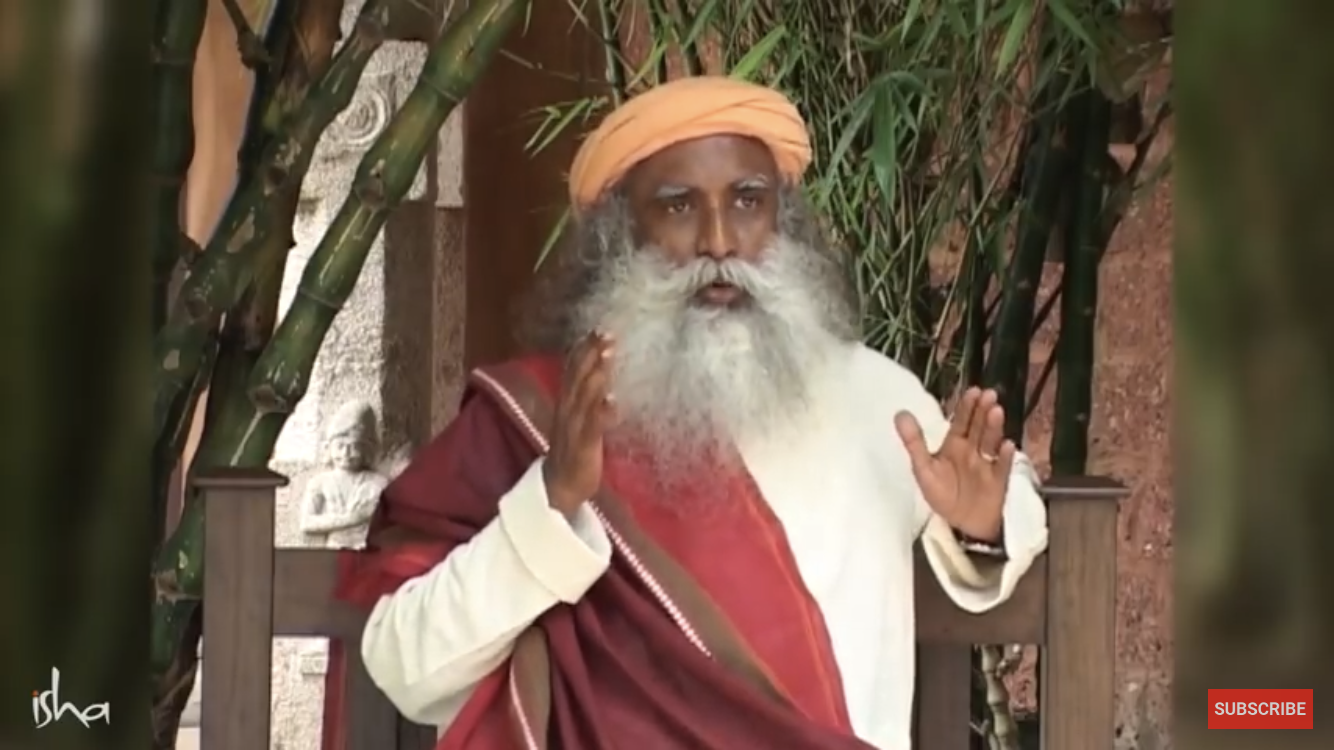
\includegraphics[width=0.5\textwidth]{tooWide}  \end{center}

\item Устаревшие заставки <<Sadhguru. Yogi, mystic and visioner.>> и <<Conversation with Mystic>> вырезаются. 

    {\color{gray}Причина: они не несут особой пользы и отнмают время.}
\end{itemize}


\subsection{Монтаж без аудио}

\begin{itemize}
\item Когда аудио-трек задерживается, иногда, монтируем в два
    этапа: один волонтер монтирует (практически) все видео, и 
    второй~--- заменяет аудио дорожку.

    В таком случае, первому монтажеру \textbf{следует оставлять 
    длинну видео-ролика неизменной}. То есть, не стоит вырезать
    фрагменты или удлинять их.

    Причина: второму человеку, обычно, будет гораздо проще 
    самому это сделать (вырезать или удлинить), чем потом сводить аудио.
\end{itemize}

\newpage
\section{Советы}\label{advices}

\subsection{Общие советы}
\textbf{Будьте внимательны~--- и не придется переделывать.}

Проверяйте, что текст без грамм. ошибок,
что все в порядки с пунктуацией;
перед монтажем проверьте в измененных фрагментах,
что все аккуратно;
после монтажа также проверьте эти места.

Измененных мест, обычно, не более 5, и это занимает 2-3 минуты,
но может сэкономить как ваше время на перерендеринг,
так и время проверяющего.

\textbf{Особое внимание}: проверьте, что не забыли замьютить
англ. аудио дорожку.

\subsection{Основные методы перевода текста.}

\begin{itemize}
    \item \emph{Наложить текст с непрозрачным бекграундом.} 

        \begin{itemize}
            \item Подходит для ситуации, когда фон в месте, где размещен текст
        одноцветен, но обычно это не так, и лучше использовать другие методы.
        \end{itemize}

    \item \emph{Наложить gaussian blur на место где находится текст, и добавить
        свой поверх.}

        \begin{itemize}
            \item Универсальный способ, подходит для 
        динамического бекграунда, и, обычно, смотрится неплохо.

            \item Ниже пример, где лучше было использовать блюр.

\begin{figure}[!hbp]
\centering
\begin{minipage}[b]{0.4\textwidth}
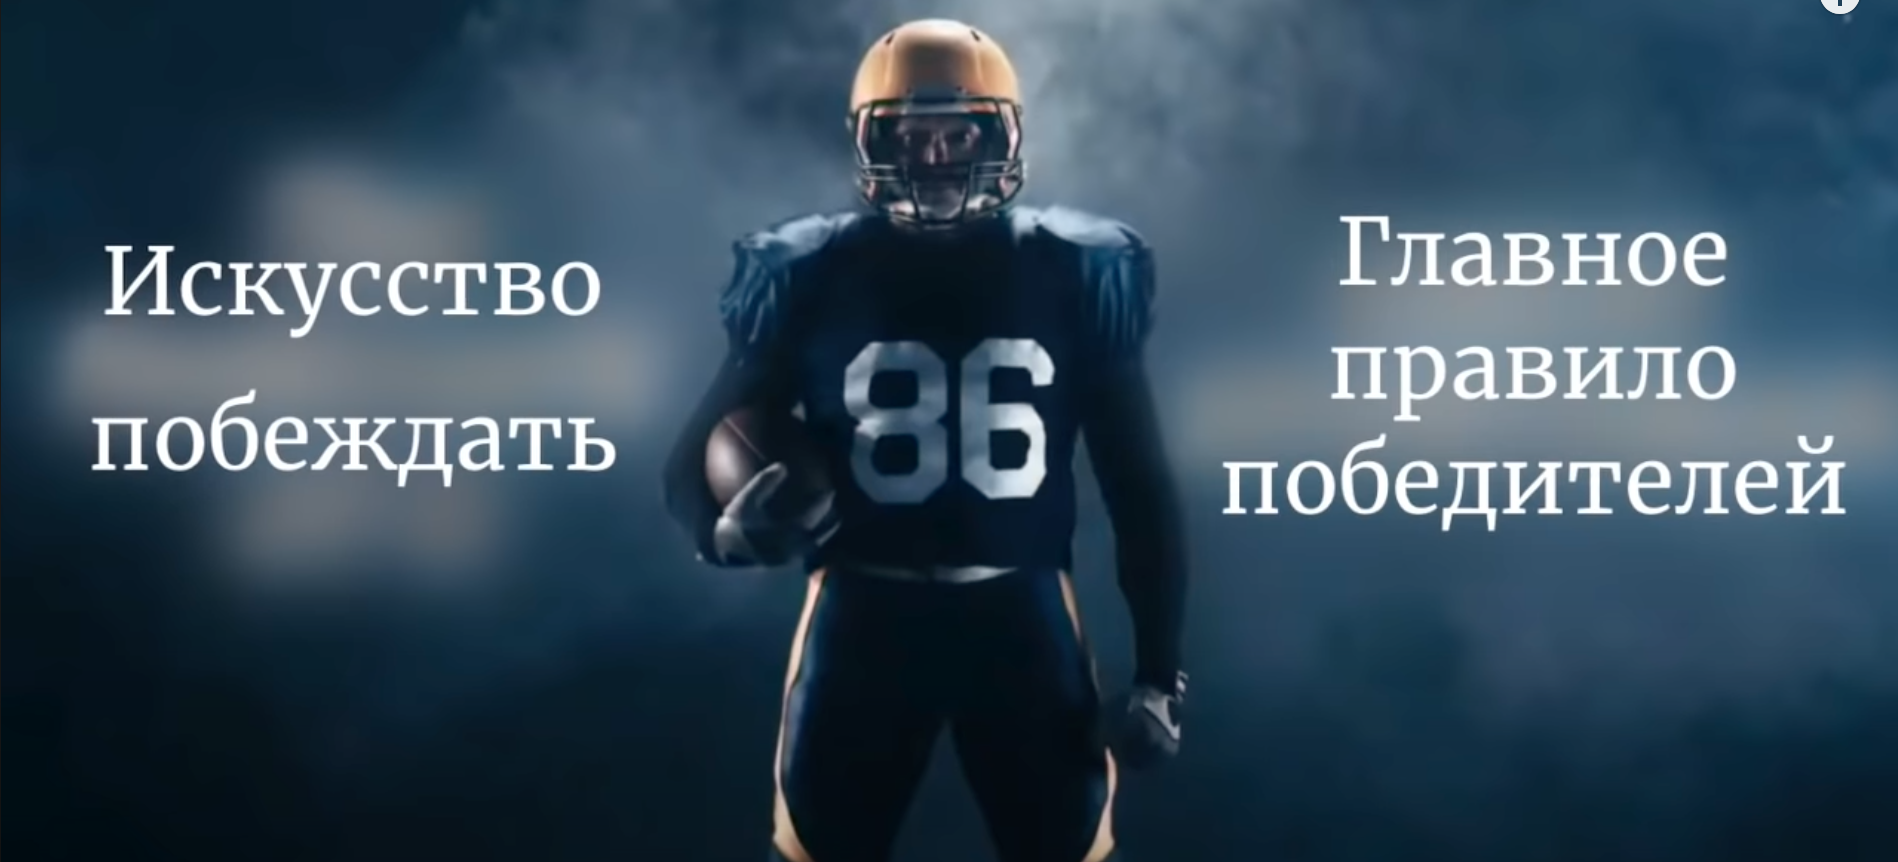
\includegraphics[width=\textwidth]{titleBlur}
\caption{Nice.}
\end{minipage}
\hfill
\begin{minipage}[b]{0.4\textwidth}

\includegraphics[width=\textwidth]{titleBlurBad}
\caption{Not nice.}
\end{minipage}
\end{figure}

        \item Если фон сливается с переведенным текстом, 
            или заблюренный английскй текст 
            добавляет слишком много белого/ черного на фон, то 
            можно добавить полупрозрачный бекграунд на переведенный текст.
    \end{itemize}

   \item \emph{Зафиксировать кадр, когда английский текст еще не появился.}

    \begin{itemize}
        \item Подходит в случае статической картинки на бэкграунде. Если 
        на заднике красивая анимация~--- blur предпочтительнее.
       
    \item Если в оригинале естть zoom (динамическое увеличение
        статической картинки) для добавления динамики, то нужно
        добавить zoom и при переводе.

    \end{itemize}
    \textit{P.S.} В обучающих материалах есть видео-пример этого способа.

\item \emph{Если есть stem (видео без английского текста).}
    
    В данном случае действуем так: скачиваем и оригинал с текстом,
    и стем. Добавляем их один поверх другого, и монтируем. В конце
    можно просто отключить (сделать невидимым) трек 
    с английским текстом.

    Для заголовков, субтитров и т.д. стараемся, по возможности,
    выбирать красивые эффекты вместо просто эффекта "Text".
\end{itemize}

\subsection{Как скачать видео} 
Чтобы скачать видео с YouTube можно воспользоваться сайтом
\href{https://www.y2mate.com/}{https://www.y2mate.com/}, скопировав и вставив 
ссылку на видео. 

Также, если видео уже открыто в браузере можно просто вставить "pp" после
слова youtube в ссылке, и y2mate откроется автоматически.

Например, https://www.youtube.com/watch?v=Oi7eLmaL1DU нужно преобразовать
в https://www.youtube\textbf{pp}.com/watch?v=Oi7eLmaL1DU .

\subsection{Где монтировать}
В Isha Foundation в основном используются Final Cut и Adobe Premiere Pro, 
однако вы можете, использовать любой удобный для вас редактор.

Например, DaVinci Resolve~---
профессиональный видеоредактор с бесплатной версией, которой нам более чем хватает. 

Для пользователей MacOS самый простой вариант монтирующей системы~--- 
iMovie, но у нее есть пара серьезных недостатков.
\begin{itemize}
    \item Нет возможности удобно добавить текст поверх видео.
        То есть, придется делать
        картинку с перевдодм в отдельном приложении и наклеивать поверх.
        Это нарушает поток, и нужно будет повозиться, если придется исправлять текст.
    \item Можно использовать только два видео трека. Это ограничивает более 
        сложных монтаж, хотя обычно двух хватает.
\end{itemize}
Поэтому совет~--- скачать более профессиональное приложение, тем более что
DaVinci бесплатный =).




\newpage
\section{Обучающие материалы}

Монтировать совсем не сложно! В начале будет немножко трудно, но основы можно 
освоить за пару часов. Главное~--- не бояться, и спрашивать, если что-то не понятно.

Так же, Google~--- ценный помошник, особенно, если гуглить на английском.
Например, запросы, вроде 
"DaVinci how to add frame hold" ("DaVinci как зафиксировать фрейм видео")
должны помочь.

Ниже real-life примеров монтажа, можете ознакомится с ними!
\begin{itemize}
    \item Подробное видео-пример монтажа видео в DaVinci. 
        Пример для ролика с YouTube, но, в 
        Instagram примерно те-же задачи)
        
        DaVinci exmple:~--- \href{https://youtu.be/SAceoBqdAvw}{https://youtu.be/SAceoBqdAvw}
    \item Короткое видео о том, как фиксировать фрейм и добавить zoom.

        DaVinci Frame Freez example:~--- \href{https://youtu.be/caPaZ5syTC8}{https://youtu.be/caPaZ5syTC8}
    \item Короткий туториал о том что делать со старыми "квадратными" видео. 

        DaVinci Narrow Video Tutorial:~--- \href{https://youtu.be/FGdErSdSOAI}{https://youtu.be/FGdErSdSOAI}

\item Три двух-минутных ролика монтажа для Instagram в Premiere Pro.

    Premiere short examples:
    \begin{itemize}
        \item \href{https://youtu.be/AWOsM9fX9RQ}{https://youtu.be/AWOsM9fX9RQ}
        \item \href{https://youtu.be/lvRnpvTXHis}{https://youtu.be/lvRnpvTXHis}
        \item \href{https://youtu.be/Ontq3mMD9AM}{https://youtu.be/Ontq3mMD9AM}
    \end{itemize}
\end{itemize}




\newpage
\section{Test Task (Тренировочное видео) YouTube}
 
Задание~--- смонтировать видео и выслать результат
ответным сообщением.. 

Вы можете загрузить видео напрямую в Telegram, или разместить
на Google Drive и присылать ссылку.

\begin{center} \textbf{Видео} \end{center}
\href{https://www.youtube.com/watch?v=9sGJUR7stzc}{Оригинал.}
\quad
\href{https://drive.google.com/file/d/1Y6ECjMSvkaUFmNawIePfFvqS2ZnB3SPi/view?usp=sharing}{Аудио трек.}
\quad
\href{https://www.youtube.com/watch?v=Q3NYDF4JyTg}{Русскоязыное видео для сравнения.}

Название видео: \textbf{Как прожить невероятную жизнь}
	
Перевод субтитра на 08:10: \textbf{<<Тайир>> на тамильском означает йогрт}


\begin{wrapfigure}{r}{0.3\textwidth}
  \begin{center}
    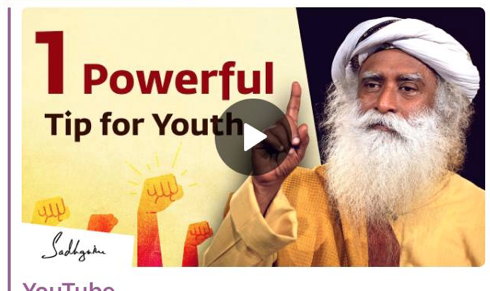
\includegraphics[width=0.28\textwidth]{thumbnail}
  \end{center}
\end{wrapfigure}

\emph{P.S.} На русском канале довольно уродливый субтитр, призываю вас улучшить его =).

\emph{P.P.S.} Thumbnail (картинка справа) делает команда дизайнеров, не монтажер.
 

\newpage
\section{Технические моменты}
\subsection{Установка шрифтов MacOs}\label{fonts}
\begin{enumerate}
    \item Скачайте шрифт, например, из Google Fonts.
    \item Откройте приложение \textbf{"font Book"}.
	    \begin{center} 
	        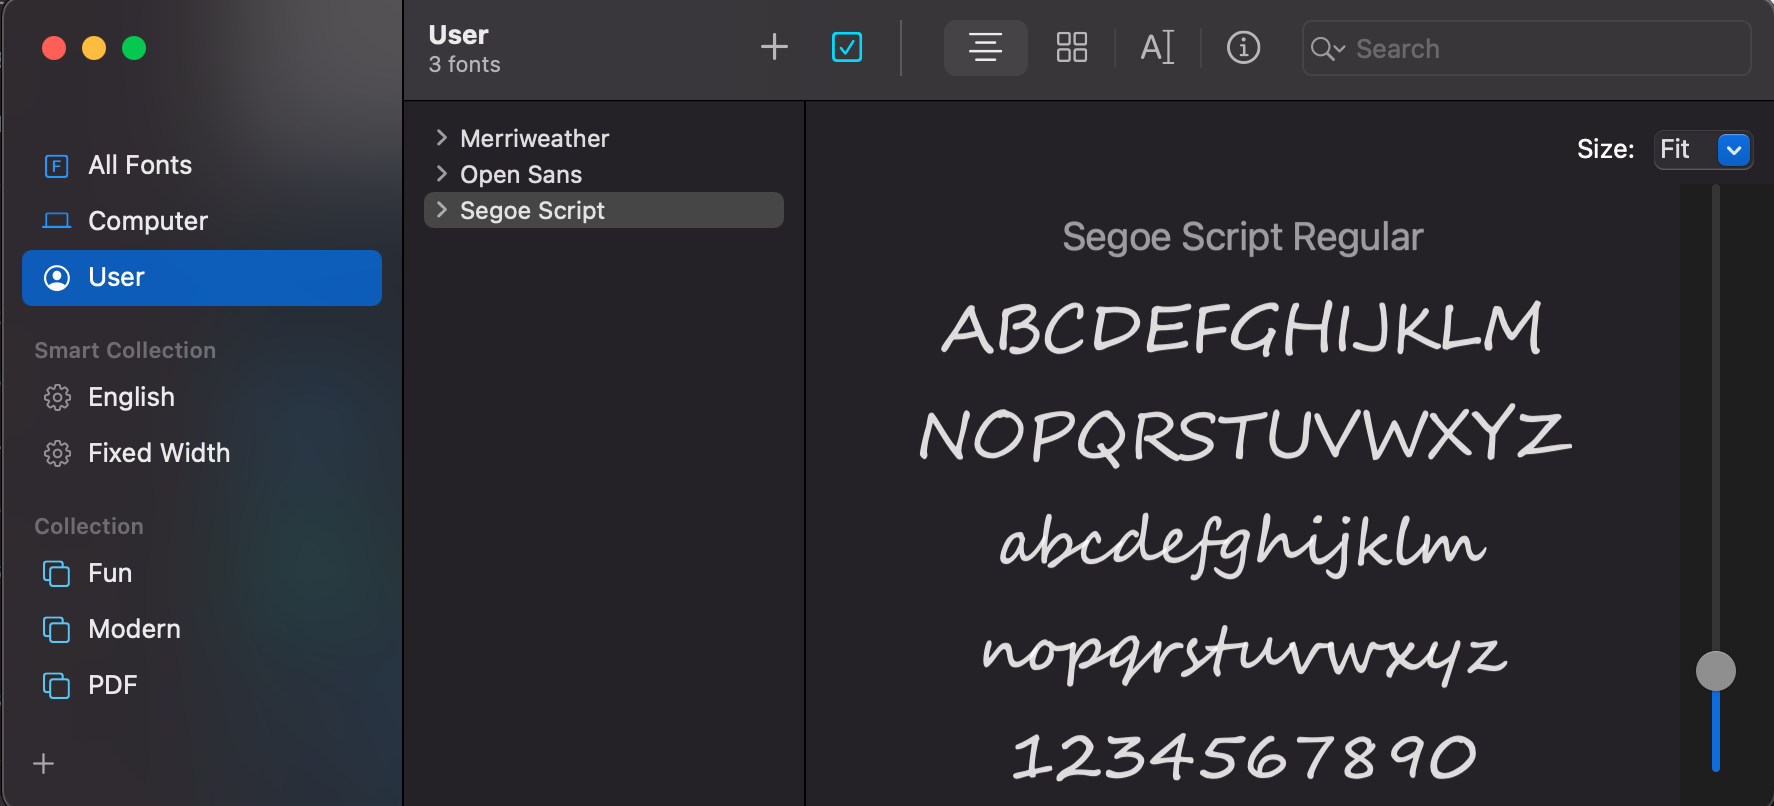
\includegraphics[width=0.9\textwidth]{fontsInstallation/macos0} 
	    \end{center}

    \item Нажмите на \textbf{"add fonts"}.
	    \begin{center} 
	        
\includegraphics[width=0.5\textwidth]{fontsInstallation/macos1} 
	    \end{center}
    \item Выберети скаченный файл и нажмите на \textbf{"Open"}.
	    \begin{center} 
	        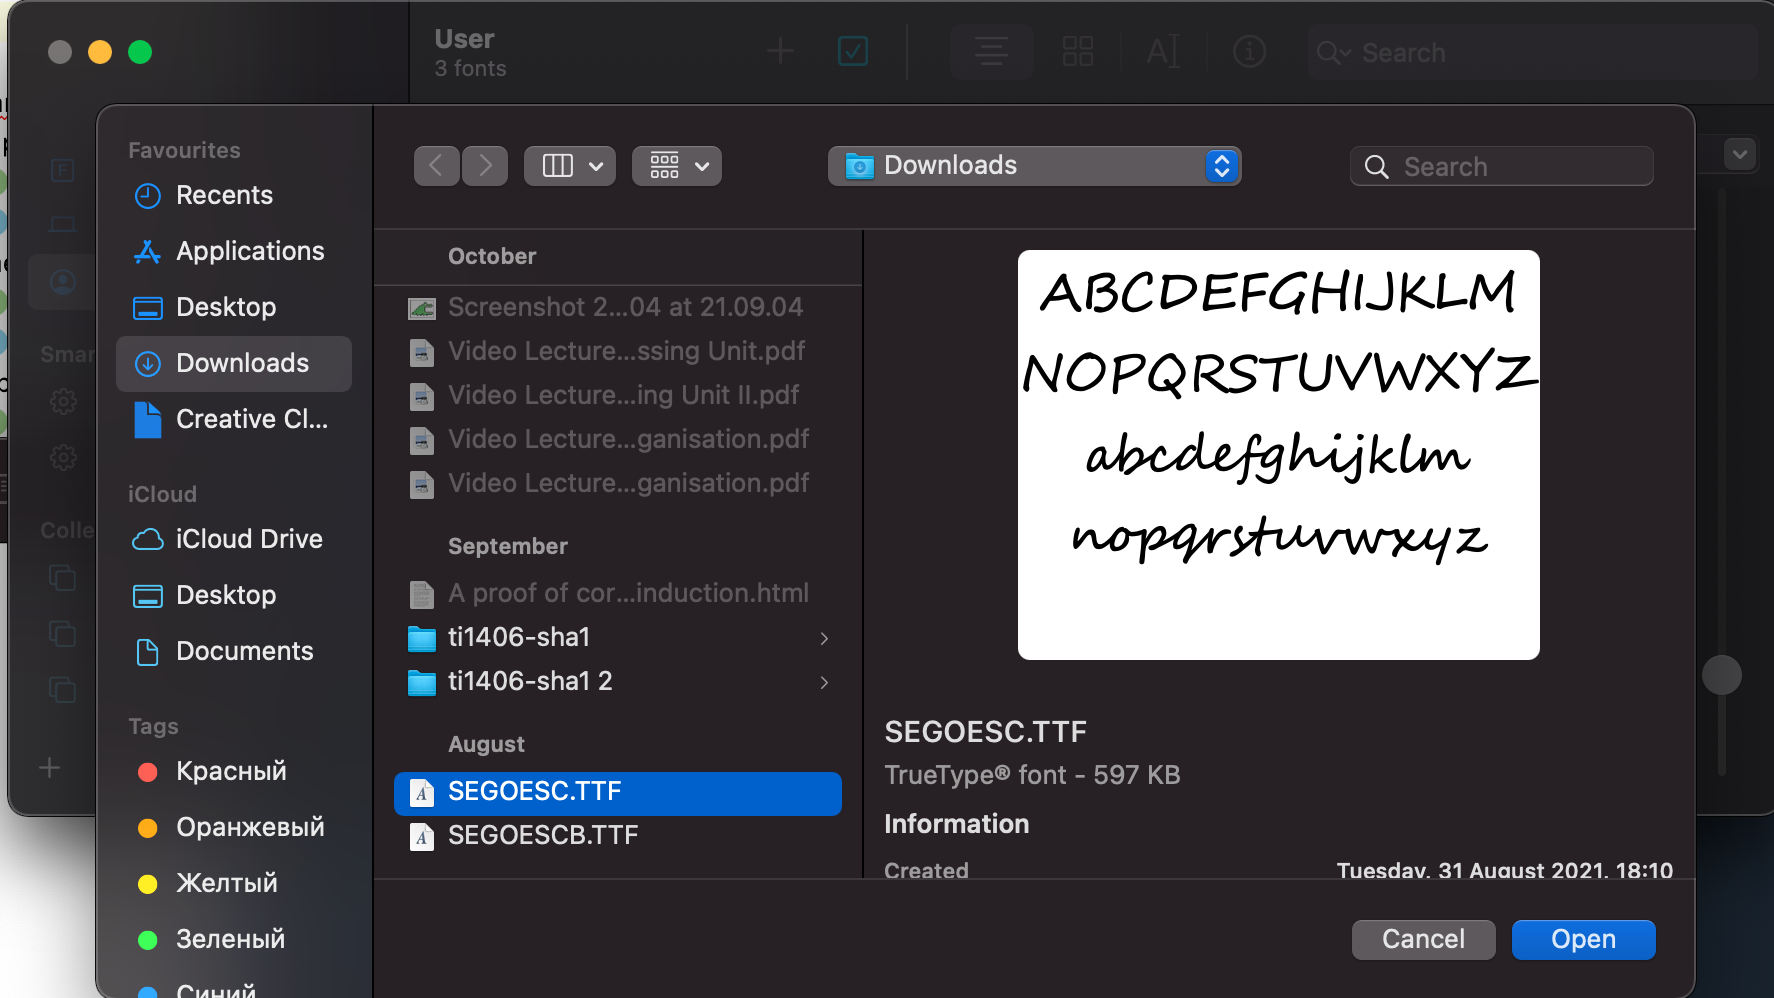
\includegraphics[width=0.9\textwidth]{fontsInstallation/macos2} 
	    \end{center}
\end{enumerate}



\newpage
\thispagestyle{empty}
\tikz[remember picture,overlay] \node[opacity=0.15,inner sep=0pt] at (current page.center){
\includegraphics[width=0.2\paperwidth]{IshaLogo}};
\end{document}
% https://www.youtube.com/watch?v=4UH7lzptFH8
